%%%%%%%%%%%%%%%%%%%%%%%%%%%%%
%% Styles, packages and new commands
\input{../Main/ML_Main.tex}
%%%%%%%%%%%%%%%%%%%%%%%%%%%%%
%% Edit the title page
\title{Machine Learning}
\subtitle{Module 7: Interpretable Machine Learning}
\author[MOB]{Marc-Olivier Boldi}
\institute[HEC MSc Mgt BA]{Master in Management, Business Analytics, HEC UNIL}
\date[Spring 2024]{Spring 2024}
%%%%%%%%%%%%%%%%%%%%%%%%%%%%%
%%%%%%%%%%%%%%%%%%%%%%%%%%%%%
%%%%%%%%%%%%%%%%%%%%%%%%%%%%%
%%%%%%%%%%%%%%%%%%%%%%%%%%%%%
\begin{document}
%%%%%%%%%%%%%%%%%%%%%%%%%%%%%
\begin{frame}
  \titlepage
\end{frame}
%%%%%%%%%%%%%%%%%%%%%%%%%%%%%
\begin{frame}
\frametitle{Table of Contents}
	\tableofcontents
\end{frame}
%%%%%%%%%%%%%%%%%%%%%%%%%%%%%
\section{Concept}
%%%%%%%%%%%%%%%%%%%%%%%%%%%%%
\begin{frame}
\frametitle{Concept}
In ML, some models are interpretable (e.g., regression, CART) and some are not (e.g., SVM, NN). \\
\vspace{0.3cm}
So called {\bf interpretable machine learning} is a set of techniques aiming at
\begin{itemize}
\item Discover / rank variables or features by their importance on the predicted outcome,
\item Associate variation of the important features with a direction of the outcome (positive vs negative association).
\end{itemize}
\end{frame}
%%%%%%%%%%%%%%%%%%%%%%%%%%%%%
\section{Variable importance}
%%%%%%%%%%%%%%%%%%%%%%%%%%%%%
\begin{frame}
\frametitle{Variable importance}
{\bf Variable importance} is a method that provides a measure of the importance of each feature for the model prediction.\\
\vspace{0.3cm}
The variables importance {\bf for a trained model} can be evaluated for one variable by:
\begin{itemize}
\item In the test set, shuffle the instances on one variable,
\item Make the predictions of this new test set,
\item Compute the quality metric (RMSE, Accuracy, ...),
\item Compare it to the quality metric on the original test set.
\item If the variable is important, giving to the model an incorrect values of this variable {\bf should decrease} the quality metric,
\end{itemize}
This is repeated for each variable.
\end{frame}
%%%%%%%%%%%%%%%%%%%%%%%%%%%%%
\begin{frame}
\frametitle{Illustration}
\begin{center}
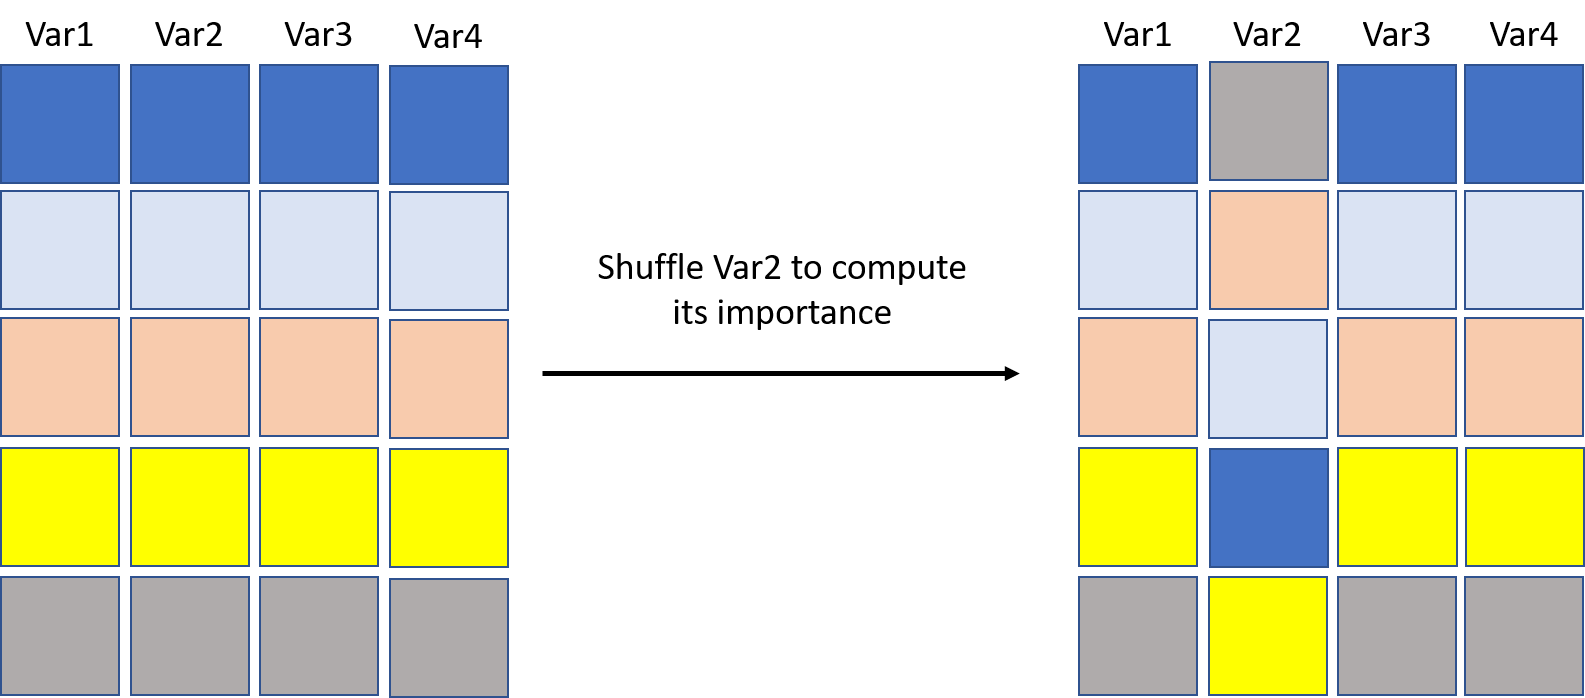
\includegraphics[width=10cm]{../Graphs/VI_Illustr.png}
\end{center}
If predictions using the right-hand side data are the same as the left-hand side ones, then Var2 is not important.
\end{frame}
%%%%%%%%%%%%%%%%%%%%%%%%%%%%%
\begin{frame}
\frametitle{Example}
With the iris data and a CART, trained on $80\%$ of the data (test set at $20\%$). The tree is
\begin{center}
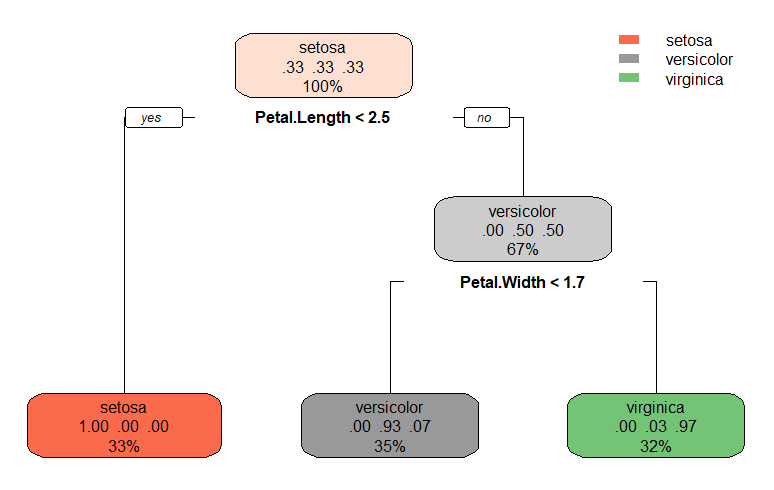
\includegraphics[width=6cm]{../Graphs/VarImp_iris_CART.png}
\end{center}
We see directly that Petal length and Petal width are the only two important features (except in case of missing data). 
\end{frame}
%%%%%%%%%%%%%%%%%%%%%%%%%%%%%
\begin{frame}
\frametitle{Example}
To measure this, in the test set, we shuffle Petal length. The accuracy of the shuffled test set is much lower than the original one (left: original test set; right: modified test set). This confirms that Petal length is essential for a good prediction of the species by the model.\\
\vspace{0.2cm}
\begin{columns}
\begin{column}{0.5\textwidth}
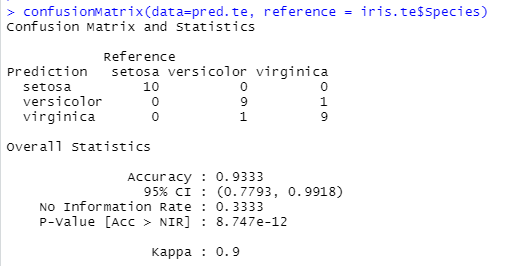
\includegraphics[width=6.5cm]{../Graphs/VarImp_iris_acc_orig.png}
\end{column}
\begin{column}{0.5\textwidth}
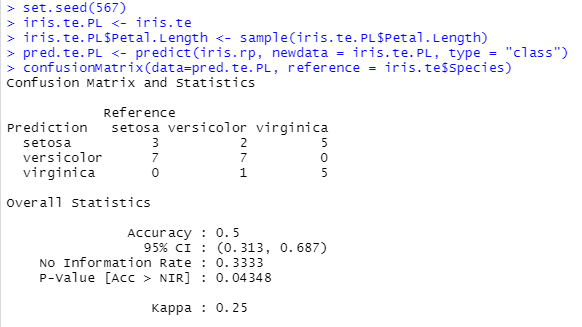
\includegraphics[width=6.5cm]{../Graphs/VarImp_iris_acc_PLsh.png}
\end{column}
\end{columns}
\end{frame}
%%%%%%%%%%%%%%%%%%%%%%%%%%%%%
\begin{frame}
\frametitle{Example}
On the other hand, the Sepal length does not appear on the graph. And, indeed, it is not important for the prediction as shown below.\\
\vspace{0.2cm}
\begin{columns}
\begin{column}{0.5\textwidth}
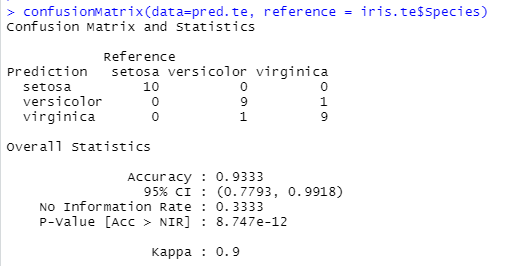
\includegraphics[width=6.5cm]{../Graphs/VarImp_iris_acc_orig.png}
\end{column}
\begin{column}{0.5\textwidth}
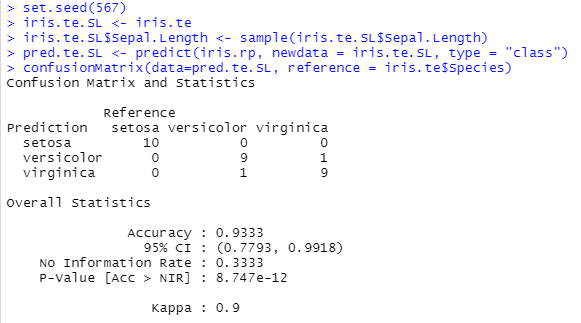
\includegraphics[width=6.5cm]{../Graphs/VarImp_iris_acc_SLsh.png}
\end{column}
\end{columns}
\end{frame}
%%%%%%%%%%%%%%%%%%%%%%%%%%%%%
\begin{frame}
\frametitle{Example}
\small
For tree, the importance of a variable can be read to some extend directly on the graph (if it is not too large). For a model like SVM, it is not. But we can still make the same analysis by shuffling the instances for a given feature (top: original; left: Petal length; right: Sepal length).
\\
\normalsize
\begin{center}
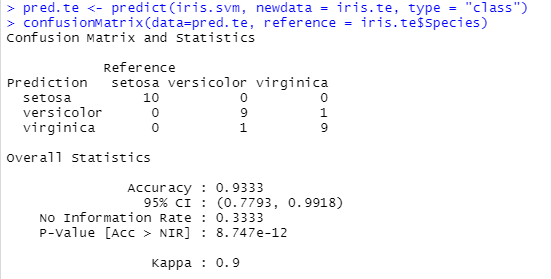
\includegraphics[width=5cm]{../Graphs/VarImp_iris_acc_svm.png}
\end{center}
\begin{columns}
\begin{column}{0.5\textwidth}
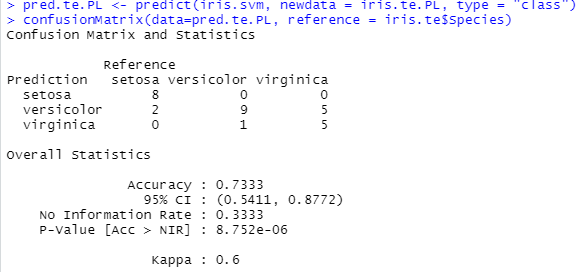
\includegraphics[width=5cm]{../Graphs/VarImp_iris_acc_svm_PL.png}
\end{column}
\begin{column}{0.5\textwidth}
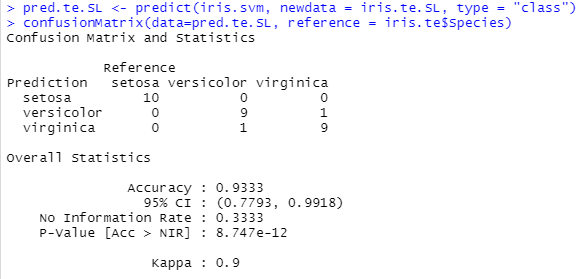
\includegraphics[width=5cm]{../Graphs/VarImp_iris_acc_svm_SL.png}
\end{column}
\end{columns}
\end{frame}
%%%%%%%%%%%%%%%%%%%%%%%%%%%%%
\begin{frame}
\frametitle{Several versions}
The variable importance presented previously is called {\bf model-agnostic}: it is independent of the model type.\\ 
\vspace{0.3cm}
There exist several ways of it:
\begin{itemize}
\item Modification of the variable: shuffling is one possibility. Perturbation is another (add a random noise). Simulation from another distribution.
\item Modification of the score: accuracy is one possibility. Specificity/Sensitivity/Bal. accuracy, Entropy... The importance can be linked to the prediction of one level only. 
\item Regression: use RMSE, MAE, etc.
\end{itemize}
\end{frame}
%%%%%%%%%%%%%%%%%%%%%%%%%%%%%
\begin{frame}
\frametitle{Model-specific VI}
There exist also {\bf model-specific} approaches that are specific to the model that is used. \\
\vspace{0.2cm}
In {\tt R}, 
\begin{itemize}
\item {\tt iml} allows to compute model-agnostic variable importance, with any loss function.
\item {\tt caret} allows to compute mainly model-specific variable importance. Also model-agnostic type (limited choice of loss functions).
\end{itemize}
\end{frame}
%%%%%%%%%%%%%%%%%%%%%%%%%%%%%
\begin{frame}[fragile]
\frametitle{Example: {\tt iml}}
VI on SVM estimated on cross-entropy, repeated 100 times.
\scriptsize
\begin{verbatim}
library(iml)
iris.iml <- Predictor$new(iris.svm, data = iris.te[,-5], y = iris.te[,5])
iris.imp <- FeatureImp$new(iris.iml, loss = "ce", n.repetitions = 100)
plot(iris.imp)
\end{verbatim}
\normalsize
\begin{center}
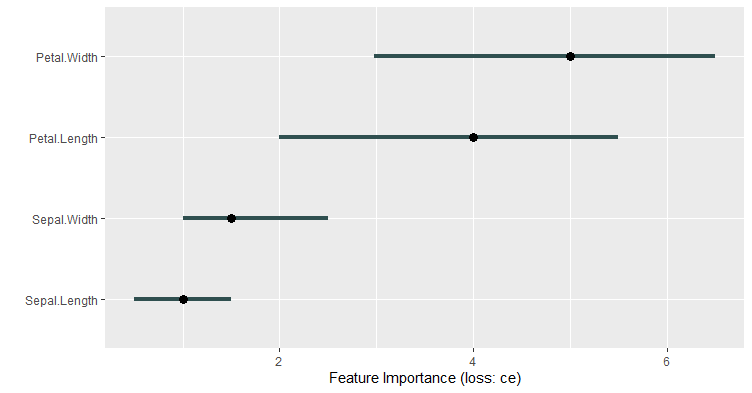
\includegraphics[width=8cm]{../Graphs/VarImp_iml_ce_svm.png}
\end{center}
\end{frame}
%%%%%%%%%%%%%%%%%%%%%%%%%%%%%
\begin{frame}
\frametitle{Example: {\tt iml}}
For each feature: The difference in entropy obtained between the original data set and the shuffled data set is computed. This is repeated 100 times. These differences are averaged and shown on the plot.
\end{frame}
%%%%%%%%%%%%%%%%%%%%%%%%%%%%%
\begin{frame}[fragile]
\frametitle{Example: {\tt caret} and {\tt VarImp}}
VI on SVM estimated on AUC.
\scriptsize
\begin{verbatim}
library(caret)
trctrl <- trainControl(method = "repeatedcv", repeats= 3, number=5)
iris.caret <- caret::train(form=Species ~., data = iris.tr, 
                    method = "svmLinear", 
                    trControl=trctrl)
plot(varImp(iris.caret))
\end{verbatim}
\normalsize
\begin{center}
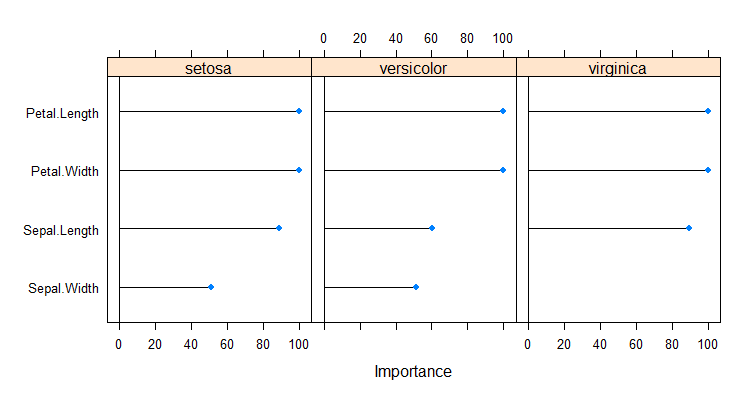
\includegraphics[width=8cm]{../Graphs/VarImp_caret_svm.png}
\end{center}
\end{frame}
%%%%%%%%%%%%%%%%%%%%%%%%%%%%%
\begin{frame}[fragile]
\frametitle{Example: {\tt caret} and {\tt VarImp}}
Since no specific method was developped for SVM, a {\bf filter-based} method is implemented. From the help of {\tt VarImp}:\\
\scriptsize
\begin{verbatim}
For classification, [...] the area under the ROC curve [...] is used 
as the measure of variable importance. For multi-class outcomes, the problem 
is decomposed into all pair-wise problems and the area under the curve is
calculated for each class pair (i.e class 1 vs. class 2, class 2 vs. 
class 3 etc.). For a specific class, the maximum area under the 
curve across the relevant pair-wise AUC's is used as the variable importance 
measure.
\end{verbatim}
\normalsize
\end{frame}
%%%%%%%%%%%%%%%%%%%%%%%%%%%%%
\begin{frame}[fragile]
\frametitle{Model-specific VI}
Even for one model, there may exist lots of implementations. Below, we give one example: {\tt VarImp} for CART. CART is recognized as {\it Recursive Partitioning} (from {\tt rpart}). From the help of {\tt VarImp}:\\
\scriptsize
\begin{verbatim}
The reduction in the loss function (e.g. mean squared error) attributed 
to each variable at each split is tabulated and the sum is returned. 
\end{verbatim}
\normalsize
\begin{itemize}
\item At each split, the reduction of loss due to the best split on each variable is extracted.
\item These loss reductions are summed. 
\end{itemize}
(No resampling or measure of error on the VI estimate)
\end{frame}
%%%%%%%%%%%%%%%%%%%%%%%%%%%%%
\begin{frame}
\frametitle{Model-specific VI}
\begin{center}
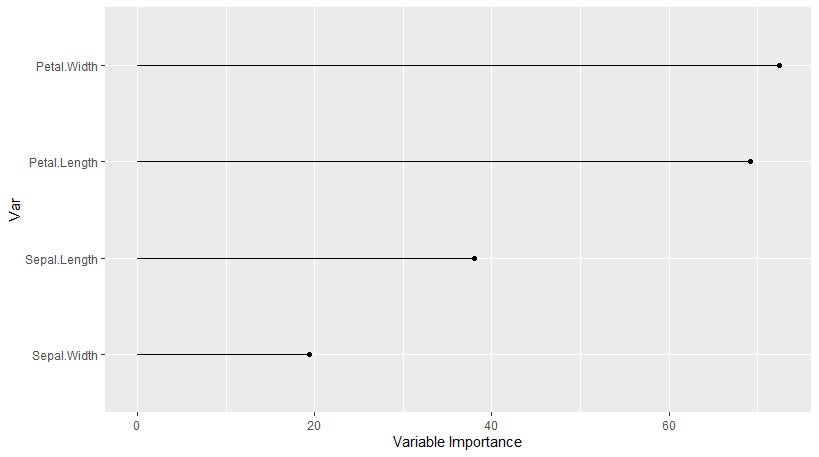
\includegraphics[width=8cm]{../Graphs/VI_iris_rp.png}
\end{center}
\end{frame}
%%%%%%%%%%%%%%%%%%%%%%%%%%%%%
\begin{frame}
\frametitle{Discussion}
Whatever implementation you use, VI aims at the same objective: quantify the importance of variables for the predictions of the model.\\
\vspace{0.3cm}
Some limitations are:
\begin{itemize}
\item {\bf Instability}: the estimation of the importance can be unstable due to the random perturbation. Resampling can help (i.e., repeat the shufling several times). 
\item {\bf Interactions}: sometimes it is the combination of two features that makes a good prediction (typ. trees). Variable importance cannot see this. 
\end{itemize}
The variable importance is only seen with {\bf the eyes of the model}. If the model is doing a poor job (e.g., low accuracy) then the variable importance analysis is of low quality.
\end{frame}
%%%%%%%%%%%%%%%%%%%%%%%%%%%%%
\section{Partial Dependence Plots}
%%%%%%%%%%%%%%%%%%%%%%%%%%%%%
\begin{frame}
\frametitle{Partial Dependence Plot}
Variable important allows to inspect how much a variable is important in the construction of the prediction by a model.\\ 
\vspace{0.2cm}
{\bf Partial dependence plots} (PDP) show in which direction is the association between a feature $x$ and the prediction of $y$. 
\end{frame}
%%%%%%%%%%%%%%%%%%%%%%%%%%%%%
\begin{frame}
\frametitle{Partial Dependence Plot}
Mathematically, for the feature $x_s$, let $f(x_s, x_{-s})$ be the prediction of $y$ by the model $f$, then the PD-function of $X_s$ at $x_s$ is
$$
F_{X_s}(x_s) = \int f(x_s, x_{-s}) p(x_{-s}) dx_{-s} = E[f(x_s, X_{-s})],
$$
where $p(x_{-s})$ is the distribution of $x_{-s}$. $F_{X_s}(x_s)$ is the expected value over $x_{-s}$ of the prediction when $x_s$ is fixed (not conditional). \\
\vspace{0.3cm}
The estimation of the expectation above is obtained by averaging on the training set:
$$
\hat{F}_{X_s}(x_s) = \frac{1}{N}\sum_{i=1}^N f(x_s, x_{-s}^{(i)}).
$$
\end{frame}
%%%%%%%%%%%%%%%%%%%%%%%%%%%%%
\begin{frame}
\frametitle{Estimation}
\begin{center}
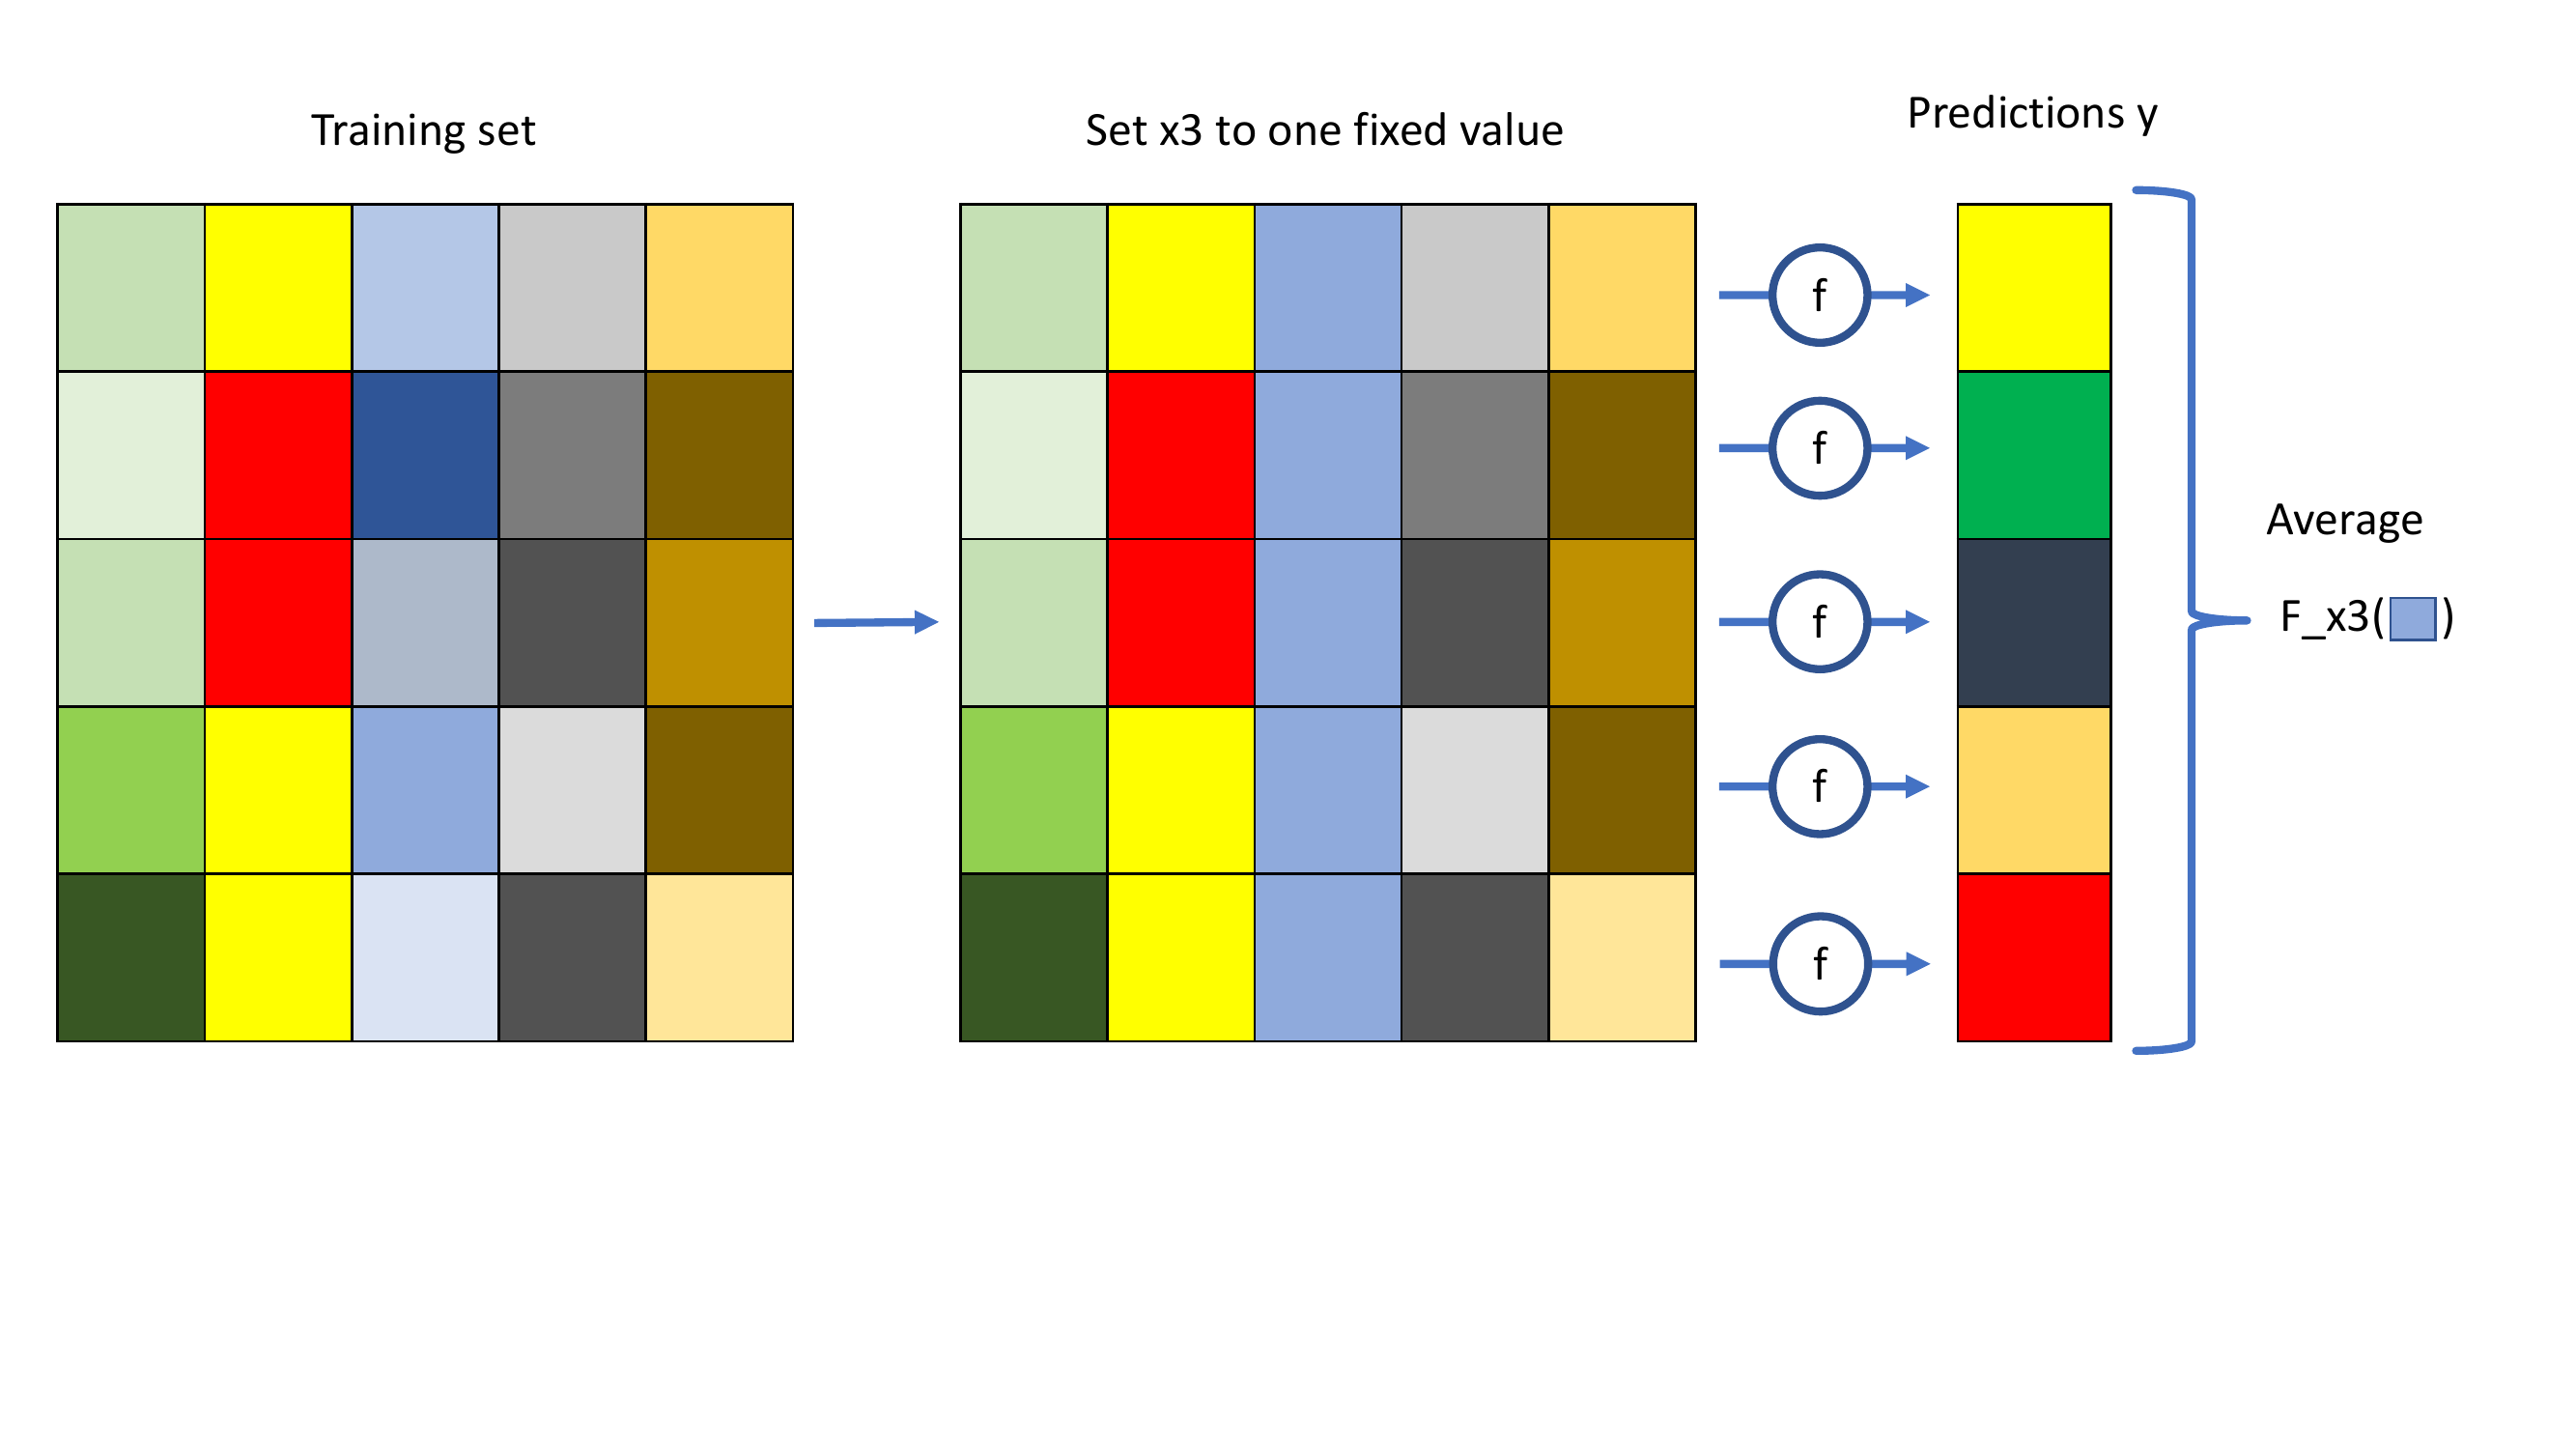
\includegraphics[width=10cm]{../Graphs/PDP_Illustr.png}
\end{center}
\end{frame}
%%%%%%%%%%%%%%%%%%%%%%%%%%%%%
\begin{frame}
\frametitle{Interpretation}
\begin{center}
\includegraphics[width=5cm]{../Graphs/PDP_Growing.png}
\includegraphics[width=5cm]{../Graphs/PDP_Stable.png}
\end{center}
\begin{itemize}
\item Left: PDP increases. The prediction increases in average when the feature increases ; it is a positive association.
\item Right: PDP is stable. The prediction does not change in average when the feature value changes; there is no association.
\end{itemize}
\end{frame}
%%%%%%%%%%%%%%%%%%%%%%%%%%%%%
\begin{frame}
\frametitle{Discussion}
\begin{itemize}
\item PDP allows to explore the link between response and any feature {\bf with the eyes of the model}.
\item PDP can be also used to see the {\bf feature importance} with the {\bf amplitude} of the graph (the larger the more important):
$$
\vert \max_{x_s} F_{X_s}(x_s) - \min F_{X_s}(x_s) \vert.
$$ 
It is richer than VI but also longer to run.
\item PDP can be made {\bf multivariate} with $X_s$ being several features (usually, max. 2).
\item By averaging, PDP {\bf ignores any interaction} between $x_S$ and $x_{-S}$.
\end{itemize}
\end{frame}
%%%%%%%%%%%%%%%%%%%%%%%%%%%%%
\section{LIME}
%%%%%%%%%%%%%%%%%%%%%%%%%%%%%
\begin{frame}
\frametitle{LIME}
LIME stands for {\bf Local interpretable model-agnostic explanations}. The paradigm is that a large ML model can be {\bf locally} approximated by an interpretable (smaller) model, a {\bf surrogate model}. 
\begin{itemize}
\item Select a instance of interest.
\item Build instances close to it and predict them.
\item Fit a surrogate model.
\item Interpret it coefficients.
\end{itemize}
\end{frame}
%%%%%%%%%%%%%%%%%%%%%%%%%%%%%
\begin{frame}
\frametitle{Illustration in 2 dimensions}
\small
On iris data, a random forest predicts setosa/virginica/versicolor from length and width (sum of the petal/sepal features). It is globally complex (left graph). Select a point of interest (blue circle). Around it (right plot), a logistic regression could be used. If you fit it on the black dots, you will find a positive association between large width and "being green", and no association with length. 
\normalsize
\begin{center}
\includegraphics[width=12cm, page=2]{../Graphs/LIME_illustr.png}
\end{center}
\end{frame}
%%%%%%%%%%%%%%%%%%%%%%%%%%%%%
\begin{frame}
\frametitle{Technical details}
There is no unique way to build/interpret surrogate models. Often,
\begin{itemize}
\item Surrogate models are linear models with variable selection.
\item The number of variables is fixed by the user.
\item Categorical features are transformed to a dummy variable: 1 if it is the same as the point of interest, 0 otherwise.
\item Numerical features are binned and dummy variables are created: 1 if it is the same bin as the point of interest, 0 otherwise.
\item Weights are assigned to sampled data according to their proximity with the point of interest (Gower's).
\end{itemize}
\end{frame}
%%%%%%%%%%%%%%%%%%%%%%%%%%%%%
\begin{frame}
\frametitle{Example}
With the bank data (see R code of examples). Three cases: Label 0 with high prob., label 1 with high prob., Label 1 with prob. $\approx 50\%$.
\begin{center}
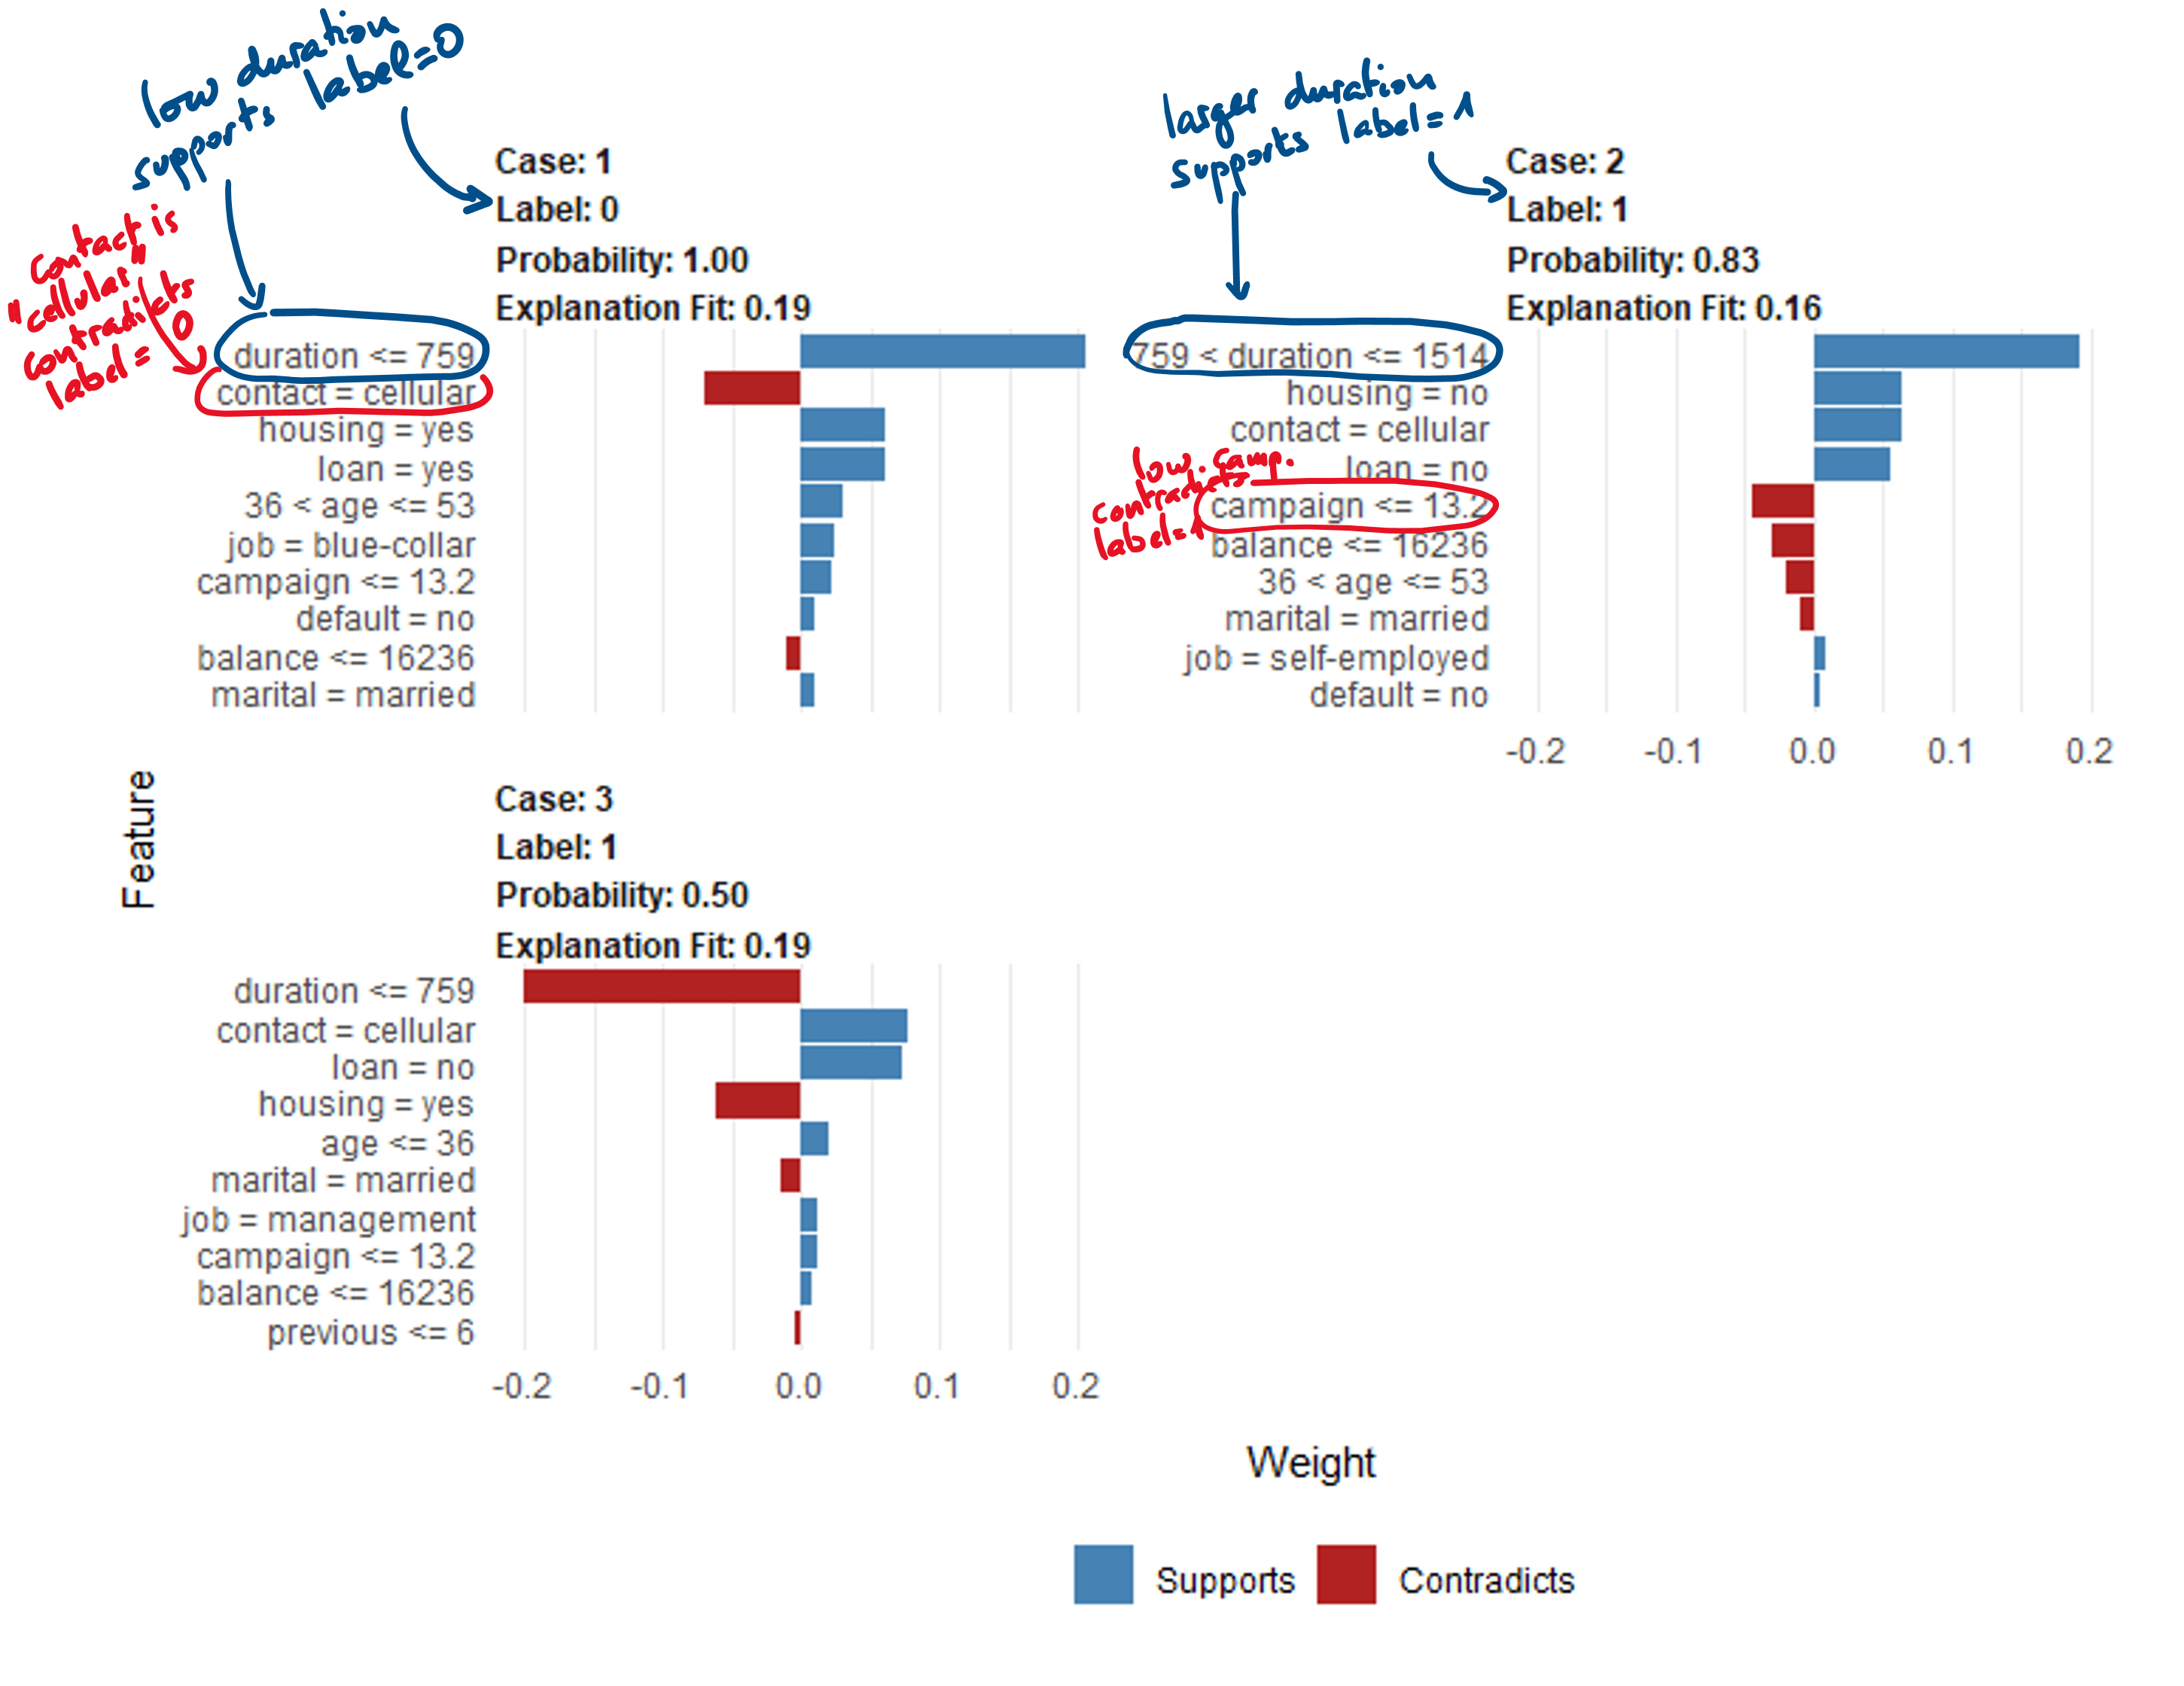
\includegraphics[width=8cm]{../Graphs/LIME_interpret.png}
\end{center}
\end{frame}
%%%%%%%%%%%%%%%%%%%%%%%%%%%%%
\begin{frame}
\frametitle{Interpretation for duration: no local behavior discovered}
\begin{itemize}
\item Around Case 1: Duration being lower than 759 supports a label 0. This means that a low duration supports label 0 and, consequently, a larger duration would support label 1. 
\item Around Case 2: Duration being greater than 759 (lower than 1514) supports label 1. This means that a large duration supports label 1 and, consequently, a lower duration would support label 0.
\item Around case 3: same as Case 2.
\end{itemize}
Regarding duration, case 1 and case 2 coincide. They also coincide with the general previous findings that duration is an important factor, with prob. of label 1 increasing with it.\\
\vspace{0.2cm}
The exploration of this two cases did not reveal any local behavior linked to duration. A similar analysis can be done for contact, housing, etc. 
\end{frame}
%%%%%%%%%%%%%%%%%%%%%%%%%%%%%
\begin{frame}
\frametitle{Interpretation for campaign: local behavior}
\begin{itemize}
\item Around Case 1: Campaign being low supports label 0. 
\item Around Case 2: Campaign being low contradicts label 1. This is in line with Case 1.
\item Around Case 3: Campaign being low supports label 1. This is in contradiction with Cases 1 and 2. 
\end{itemize}
This example shows that a global behavior (campaign is positively associated with label 1) can change locally. The fact that Case 3 has a probability around 0.5 makes it interesting. \\
\vspace{0.2cm}
Limitation: here the effect of Campaign is so small that a good explanation is that it has almost no effect everywhere. That was just a toy example.
\end{frame}
%%%%%%%%%%%%%%%%%%%%%%%%%%%%%
\begin{frame}
\frametitle{Discussion}
\begin{itemize}
\item The choice of the point of interest can be anything, even non-observed instances. Average, extreme, and change points are often of interest.
\item This method interprets locally the link between the features and the response, again, with the eyes of the model.
\item The surrogate models (as well as the global model) cannot support rigorous causal analysis. We can discover only association here. 
\item Like often, this method can be unstable (implementation, choice of the model, etc.). Try several combinations and be cautious with conclusions.
\end{itemize}
\end{frame}
%%%%%%%%%%%%%%%%%%%%%%%%%%%%%
%%%%%%%%%%%%%%%%%%%%%%%%%%%%%
\end{document}

\begin{frame}[fragile]
\frametitle{Model-specific VI}
\tiny
\begin{verbatim}
> summary(iris.rp)
[...]
Node number 1: [...]
  Primary splits:
      Petal.Length < 2.5  to the left,  improve=40.00000, (0 missing)
      Petal.Width  < 0.8  to the left,  improve=40.00000, (0 missing)
      Sepal.Length < 5.45 to the left,  improve=27.88515, (0 missing)
      Sepal.Width  < 3.35 to the right, improve=15.20000, (0 missing)
[...]
Node number 3: [...]
  Primary splits:
      Petal.Width  < 1.65 to the left,  improve=32.48120, (0 missing)
      Petal.Length < 4.75 to the left,  improve=29.19192, (0 missing)
      Sepal.Length < 6.15 to the left,  improve=10.10101, (0 missing)
      Sepal.Width  < 2.95 to the left,  improve= 4.24890, (0 missing)
[...]


> varImp(iris.rp)
              Overall
Petal.Length 69.19192
Petal.Width  72.48120
Sepal.Length 37.98616
Sepal.Width  19.44890
\end{verbatim}
\end{frame}
%%%%%%%%%%%%%%%%%%%%%%%%%%%%%
